\chapter{Media Item Deduplication}
\label{sec:media-item-deduplication}

% the code below specifies where the figures are stored
\ifpdf
    \graphicspath{{6_media_item_deduplication/figures/PNG/}{6_media_item_deduplication/figures/PDF/}{6_media_item_deduplication/figures/}}
\else
    \graphicspath{{6_media_item_deduplication/figures/EPS/}{6_media_item_deduplication/figures/}}
\fi

\section{Introduction}

In the previous \autoref{cha:media-item-extraction}
in \autoref{sec:the-need-for-media-item-deduplication},
we have motivated the need for media item deduplication.
By clustering media items, we get a~higher-level view on
a~media item cluster's overall performance on different networks.
As detailed in \autoref{sec:definition}, media items can be
photos or videos.
WordNet~\cite{fellbaum1998wordnet,miller1995wordnet} defines
the term \emph{duplicate} as
\textit{``a copy that corresponds to an original exactly''}.
The corresponding verb \emph{to duplicate} is defined as to
\textit{``make a~duplicate or duplicates of''}.
The derived term \emph{deduplication} in consequence refers to
the act of eliminating duplicate or redundant information.

\subsection{Definition of Exact Duplicate for Photos}

We define two media items of type photo as \emph{exact duplicate}
if their pixel contents are exactly the same.
This implies that by our definition, a~scaled or recompressed version
of the same photo is \emph{not} an exact duplicate. 
Similarly, a~rotated version of a~photo is also \emph{not}
an exact duplicate. 
In contrast, two photo files with different file names
or different Exchangeable image file
format\footnote{\url{http://www.cipa.jp/english/hyoujunka/kikaku/pdf/DC-008-2010_E.pdf},
accessed November 22, 2012}
(Exif) data are considered exact duplicate
if their pixel contents are exactly the same.
Exact duplicate photos typically occur if users share content 
from one social network on another, for example,
if one user posts a~photo on Instagram that then someone else
(or even the same user) posts on Facebook.

\subsection{Definition of Near-Duplicate for Photos}

We define two media items of type photo as \emph{near-duplicate}
if their pixel contents differ no more than a~given threshold after resampling.
Examples of near-duplicate photos are scaled versions
of the same photo, photos shot from a~slightly different angle,
rotated photos up to a~certain degree, \emph{etc.}
Near-duplicate photos typically occur if event attendants
stand close to each other and thus take photos
from a~similar standpoint.
Another scenario is a~user applying a~photo effect to a~photo
(like an Instagram filter) and then sharing both the modified
and the unmodified version.

\subsection{Definition of Exact Duplicate for Videos}

We define two media items of type video as \emph{exact duplicate}
if their pixel contents are frame by frame exactly the same.
In practice, we lower this condition and instead of every frame
only consider frames at shot boundaries.
We make \emph{no} requirements on the audio, \emph{i.e.},
a video in two different languages, however, that fulfills the 
pixel contents equality condition, is considered exact duplicate.
Typical scenarios where exact duplicate videos can occur is,
for example, two users sharing the same YouTube video
independently from each other.

\subsection{Definition of Near-Duplicate for Videos}

We define two media items of type video as \emph{near-duplicate},
if their pixel contents per frame differ no more
than a~given threshold.
In practice, we lower this condition and instead of every frame
only consider frames at shot boundaries.
Typical scenarios where near-duplicate videos can occur is through
logo or subtitle insertion, resizing, re-encoding,
or aspect-ration changes.
Note that we do not consider video subsegments near-duplicates.

\subsection{Special Case of Photo Contained in a~Video}

We define the special case of
\emph{a photo being contained in a~video} if the pixel contents
of a~photo media item differ no more than a~given threshold from
the pixel contents of any of the frames of a~video media item.
In practice, we lower this condition and instead of every frame
only consider frames at shot boundaries.
Typically, this phenomenon occurs if two event attendants
of the same event both cover the event from almost the same
standpoint, however, if the one attendant takes a~video,
while the other attendant takes a~photo.

\subsection{Motivation and Chapter Outline}

In this chapter, we will treat video
and photo deduplication separately. 
Our goal is to deduplicate media items on-the-fly
at the very moment they are extracted from social networks.
Due to this limitation, we cannot rely on any preprocessing
at all that state-of-the-art algorithms rely on.
This is why we dedicate a~whole section entirely to on-the-fly
shot boundary detection for online video,
which is by no means a~solved problem.
The contribution of our approach is that it is entirely Web-based
and on-the-fly, which introduces interesting new challenges
that traditional approaches to shot boundary detection
do not have to cope with.
Our Web-based approach abstracts away most of the low-level details
like the video codec, in favor of the high-level \texttt{<video>}
API, however, this also comes at a~cost.
A~major issue is the uncertain streaming speed,
where traditional approaches have immediate access
to the video file on disk.
An additional challenge is the unknown key frame distribution
of the target videos, which---together with streaming speed
issues---makes exact frame-wise video navigation impossible.
Our approaches to video and photo near-duplicate
and exact duplicate detection are founded
on a~tile-wise histogram-based pixel comparison algorithm.

\section{Video Shot Boundary Detection}
Video shot boundary detection is the for machines processor-intensive task
of splitting a~video into continuous camera shots,
with hard or soft cuts as the boundaries.
In this section, we present a~browser-based, client-side, and
on-the-fly approach to this challenge
based on modern HTML5~\cite{berjon2012html5} Web APIs.
Once a~video has been split into shots,
shot-based video navigation becomes enabled,
more fine-grained playing statistics can be created,
and finally, shot-based video comparison is possible.
\autoref{fig:screenshot} shows detected camera
shots for a~sample video.
The algorithm has been incorporated in a~browser extension
so that it can run transparently on a~major online video portal.

\begin{figure}
  \begin{center}
    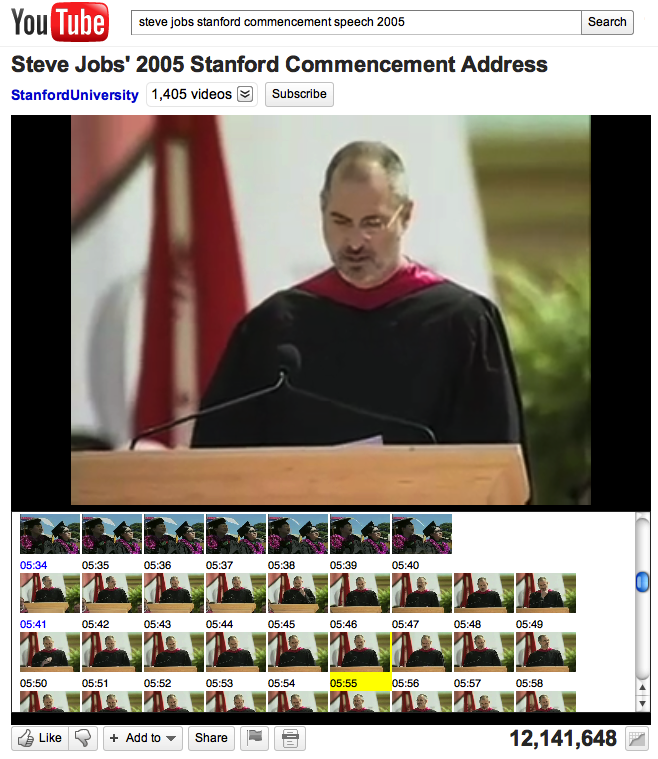
\includegraphics[width=0.7\linewidth]{./stevejobs.png}
  \end{center}
  \caption[Camera shots for a~sample video on  
    a~major online video portal]
    {Camera shots for a~sample video on 
    a~major online video portal, detected on-the-fly via
    our shot boundary algorithm incorporated
    in a~browser extension.}
  \label{fig:screenshot}
\end{figure}

\subsection{Related Work} \label{sec:related-work}
Video fragments consist of shots, which are sequences of
consecutive frames from a~single viewpoint,
representing a~continuous action in time and space.
The topic of shot boundary detection has already been described
extensively in literature.
While some specific issues still remain
(notably gradual transitions and false positives
due to large movement or illumination changes),
the problem is considered resolved for many
cases~\cite{yuan2007shotboundary,hanjalic2002shotboundary}.
Below, we present an overview of several well-known categories of shot boundary detection techniques.

\emph{Pixel comparison
methods}~\cite{hampapur1994videosegmentation,
zhang1993videopartitioning} construct a~discontinuity metric
based on differences in color or intensity values
of corresponding pixels in successive frames.
This dependency on spatial location makes this technique
very sensitive to (even global) motion.
Various improvements have been suggested, such as prefiltering
frames~\cite{zhang1995videoparsing},
but pixel-by-pixel comparison methods proved inferior in the end
and have steered research towards other directions.

A~related method is
\emph{histogram analysis}~\cite{otoole1999shotboundary},
where changes in frame histograms are used
to justify shot boundaries.
Their insensitivity to spatial information
within a~frame makes histograms less prone to partial
and global movements in a~shot.

As a~compromise, a~third group of methods consists of
a~\emph{trade-off between the above two
techniques}~\cite{ahmed1999keyframe}.
Different histograms of several, non-overlapping blocks
are calculated for each frame,
thereby categorizing different regions of the frame
with their own color-based, space-invariant fingerprint.
The results are promising, while computational complexity
is kept to a~minimum, which is why we have chosen
a~variation of this approach for our own algorithm.

Other approaches to shot boundary detection include
the \emph{comparison of mean and standard deviations}
of frame intensities~\cite{lienhart1999comparison}.
Detection using other features such as
edges~\cite{zabih1995scenebreaks} and
motion~\cite{bouthemy1997shotchange} have also been proposed.
However, Gargi \emph{et~al.} have shown that
these more complex methods do not necessarily
outperform histogram-based approaches~\cite{gargi2000videoshot}.
A~detailed comparison can be found in
Yuan~\emph{et~al.}~\cite{yuan2007shotboundary}.

\subsection{Shot Boundary Detection Algorithm}
\label{sec:details-of-algo}

In this section, we discuss our shot boundary detection algorithm,
which falls in the category of histogram-based algorithms.
Since visually dissimilar video frames
can have similar global histograms,
instead we take local histograms into account. 
We therefore split video frames in freely configurable
rows and columns, \emph{i.e.}, lay a~grid of tiles over each frame.
The user interface, as can be seen in \autoref{fig:algorithm},
currently allows for anything from a~$\mathit{1} \times \mathit{1}$ 
grid to a~$\mathit{20} \times \mathit{20}$ grid.
The limits are imposed by still reasonable processing time on consumer PCs.
For each step, we examine a~frame $\mathit{f}$ and its direct
predecessor frame $\mathit{f - 1}$.

Apart from the per-tile average histogram distance,
the frame distance function further considers
a~freely configurable number of \emph{most different} and
\emph{most similar} tiles.
This is driven by the observation that different parts
of a~video have different intensities of color changes,
dependent on the movements from frame to frame.
The idea is thus to boost the influence of movements in the frame
distance function, and to limit the influence of permanence.
In the debug view of our approach, as depicted in
\autoref{fig:algorithm}, blue boxes indicate movements,
while red boxes indicate permanence.
In the concrete example, Steve Jobs' head and shoulders move
as he talks, which can be clearly seen
at the blue boxes in the particular tiles.
Additional movements come from a~swaying flag on the left,
and a~plant on the right.
In contrast, the speaker desk, the white background,
and the upper part of his body remain static,
resulting in red boxes.
For this example, we use a~grid layout of
$\mathit{20} \times \mathit{20}$ tiles
($\mathit{nTiles} = \mathit{400}$),
and an empirically determined  number
$\mathit{tileLimit}$ of most different or similar tiles,
\emph{i.e.}, we treat one third of all tiles
as most different tiles, one third as normal tiles,
and one third as most similar tiles,
and apply boosting and limiting factors to the most different
and most similar tiles respectively.
We work with values of~$\mathit{1.1}$ for the
$\mathit{boostingFactor}$, which slightly increases
the impact of the most different tiles,
and $\mathit{0.9}$ for the $\mathit{limitingFactor}$,
which slightly decreases the impact of the most similar tiles.
The algorithm pseudo code can be seen in \autoref{code:algorithm}.

We define the average histogram distance between two frames
$\mathit{f}$ and $\mathit{f - 1}$ as $\mathit{avgHisto}_{f}$.
In a~first step, we have examined the histogram distance
data statistically, and observed that while
the overall average frame distance $\mathit{avgDist}_{f}$,
defined as $$\mathit{avgDist}_{f} =
\frac{1}{\mathit{nTiles}}\sum_{t=1}^{\mathit{nTiles}}
\mathit{avgHisto}_{f, t}$$ is very intuitive to human beings,
far more value lies in the standard deviation
$\mathit{stdDev}_{f}$, based on the definition of the overall
average frame distance $\mathit{avgDist}_{f}$
$$\mathit{stdDev}_{f} =
\sqrt{\frac{1}{\mathit{nTiles}}\sum_{t=1}^{\mathit{nTiles}}
(\mathit{avgHisto}_{f, t} - \mathit{avgDist}_{f})^{2}}$$
We use the standard deviation as a~value for the shot splitting
threshold~\cite{lienhart1999comparison}
to come to very accurate shot splitting results.
We found the boosting and limiting factors to have an overall
positive quality impact on more lively videos,
and a~negative quality impact on more monotone videos.
Best results can be achieved if,
after changing either the boosting or the limiting factors
for the most similar or different tiles,
the value of the shot splitting threshold is adapted
to the new resulting standard deviation.
The user interface optionally does this automatically.

\begin{figure}
  \begin{center}
    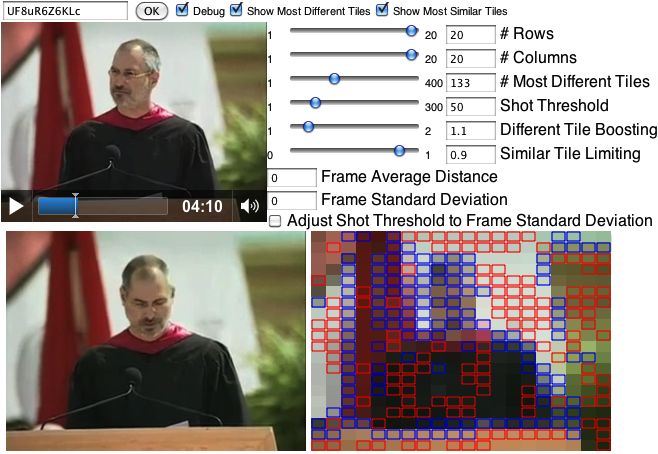
\includegraphics[width=1.0\linewidth]{./algorithm.png}
  \end{center}
  \caption[Debug view of the shot boundary detection process]
    {Debug view of the shot boundary detection process.
    Blue boxes highlight tiles with the most differences
    to the previous frame, red boxes those with most similarities.}
  \label{fig:algorithm}
\end{figure}

\begin{lstlisting}[caption=Pseudocode of shot boundary detection
  algorithm.,
  label=code:algorithm, float]
for frame in frames
  f = frame.index  
  for tile in tiles of frame      
    avgHisto[f][tile] = getTilewiseDiff()
 
  mostDiffTiles = getMostDiffTiles(avgHisto[f])
  mostSimTiles = getMostSimTiles(avgHisto[f])
 
  for tile in tiles of frame    
    factor = 1  
    if tile in mostDiffTiles
      factor = boostingFactor
    else if tile in mostSimTiles
      factor = limitingFactor
    avgHisto[f][tile] = avgHisto[f][tile] * factor
  avgDist[f] = avg(avgHisto[f])
\end{lstlisting}

\subsection{Implementation Details}
\label{sec:implementation}

The complete video analysis process happens fully
on the client side.
We use HTML5 JavaScript APIs of the \texttt{<video>} and
\texttt{<canvas>} tags.
In order to obtain a~video still frame
from the \texttt{<video>} tag at the current video position,
we use the \texttt{drawImage()} function of the 2D context of the
\texttt{<canvas>} tag,
which as its first parameter accepts a~video.
We then analyze the video frame's pixels tile-wise
and calculate the histograms.
In order to retrieve the tile-wise pixel data
from the 2D context of the \texttt{<canvas>},
we use the \texttt{getImageData()} function.
For processing speed reasons, we currently limit our approach to
a~resolution of one second, \emph{i.e.},
for each analysis step,
seek the video in $\mathit{1s}$ steps.
We then calculate the frame distances as outlined in
\autoref{sec:details-of-algo}.
For each frame, we can optionally generate an \texttt{<img>} tag
with a~base64-encoded data URI representation
of the video frame's data
that can serve for filmstrip representations of the video.

\subsection{Evaluation} \label{sec:evaluation}

Detecting shots on-the-fly in streaming video
comes with its very own challenges.
First, it is a~question of streaming speed.
Especially with high-definition (HD) video,
this can be very demanding.
We do not attach the analysis \texttt{<video>} tag
to the DOM tree~\cite{lehors2004dom} to save some CPU cycles,
however, the video still needs to be sought to each frame
in one-second steps and be processed.
Even on a~higher-end computer (our experiments ran on a~MacBook
Pro, Intel Core 2 Duo 2,66 GHz, 8 GB RAM),
the process of analyzing and displaying in parallel
a~$\mathit{1280} \times \mathit{720}$ HD video of media type
\emph{video/mp4; codecs="avc1.64001F, mp4a.40.2"}
caused an average CPU load of about 70\%.
The HTML5~\cite{berjon2012html5} specification states that
\textit{``when the playback rate is not exactly 1.0,
hardware, software, or format limitations can cause video frames
to be dropped''}.
In practice, this causes the analysis environment
to be far from optimal.
In our experiments we differentiated between false positives,
\emph{i.e.}, shot changes that were detected,
but not existent, and misses, \emph{i.e.},
shot changes that were existent,
but not detected.
Compared to a~set of videos with manually annotated shot changes,
our algorithm detected fewer false positives than misses.
The reasons were gradual transitions and shots
shorter than one second (below our detection resolution)
for misses, and large movements in several tiles
for false positives.
Overall, we reached an accuracy of about 86\%,
which is not optimal, but given the challenges
sufficient for our use case of
detecting near- or exact duplicate videos. 

\subsection{Optimization Potential}

Optimization potential lies in
improving the analysis speed by dynamically selecting
lower quality analysis video files,
given that videos are oftentimes available in several resolutions,
like Standard Definition (SD) or High Definition (HD).
We have checked in how far analysis results differ
for the various qualities,
with the result that SD quality is sufficient.
Second, more advanced heuristics for the various user-definable
options in the analysis process are needed.
While there is no optimal configuration for all types of videos,
there are some key indicators that can help categorize videos
into classes and propose predefined known working settings
based on the standard deviation $\mathit{stdDev_{f}}$
and the overall average frame distance $\mathit{avgDist_{f}}$.
Both are dependent on the values of $\mathit{boostingFactor}$,
$\mathit{limitingFactor}$, $\mathit{rows}$, and $\mathit{columns}$. 
Interpreting our results so far, there is evidence
that low complexity settings are sufficient in most cases,
\emph{i.e.}, a~number of $\mathit{rows}$ and $\mathit{columns}$
higher than~$\mathit{2}$ does not necessarily
lead to more accurate shot boundary detection results.
The same applies to the number of to-be-considered most different
or similar tiles $\mathit{tileLimit}$.
We had cases where not treating those tiles differently
at all, \emph{i.e.}, setting
$\mathit{boostingFactor} = \mathit{limitingFactor} = \mathit{1}$, 
led to better results.

\section{Photo Deduplication}

We determine the popularity of media items
shared across social networks.
This task involves the deduplication of extracted media items.
In the previous section, we have presented an algorithm
for on-the-fly shot boundary detection for video media items.
In this section, we will show how components of this algorithm
can be used to deduplicate photos.
First, we look at related work for the task of photo deduplication.

\subsection{Related Work}

Work on ordinal measures that serve as a~general tool for
image matching was performed by Bhat \emph{et al.}\
in~\cite{bhat1998imagecorrespondence}.
Chum \emph{et al.}\ have proposed a~near-duplicate image detection method
using min-Hash and term frequency--inverse document frequency (tf--idf)
weighting~\cite{chum2008nearduplicate}.
The proposed method uses a~visual vocabulary of
vector quantized local feature descriptors based on
Scale Invariant Feature Transform (SIFT)~\cite{lowe1999sift}.
A~method for both photos and videos~\cite{yang2009nearduplicate}
has been proposed by Yang \emph{et al.}

\subsection{Duplicate Content}
\label{sec:duplicate-content}

Duplicate content in the context of social networks
arises whenever people either share exactly the same,
or an exact copy of a~given media item.
An example of the latter can be one user uploading the same media item
to the two different social networks \googleplus and Facebook,
and an example of the prior can be two users sharing the same
YouTube video independently from each other, or re-sharing each other's content.

\subsubsection{Near-Duplicate Content}

Near-duplicate content in the context of social networks
arises in a~number of situations
that we will illustrate in the following.
All photos are real examples of media items shared on social networks
that were clustered correctly as near-duplicates
by our clustering algorithm, which we will detail in
\autoref{sec:near-duplicate-clustering-algorithm}.

\paragraph{Different Viewing Angle}

When two people attend the same event
and produce media items at roughly the same time
covering the same scenes,
their media items will be similar
and only differ in the viewing angle. 
\autoref{fig:viewing-angle} shows a~concrete example.

\begin{figure}[h!]
  \centering
  \subfloat[Viewing angle 1]{
    
\includegraphics[width=0.25\textwidth]{stage1.jpg}
  }                
  \subfloat[Viewing angle 2]{
    
\includegraphics[width=0.25\textwidth]{stage2.jpg}
  }
  \caption{Slightly different viewing angles of a~concert stage.}
  \label{fig:viewing-angle}  
\end{figure}

\paragraph{Logo, Watermark, Lower Third, or Caption Insertion}

Oftentimes organizations or individuals insert
logos, watermarks, or captions into media items
to highlight their origin or convey related information,
or to claim ownership of a~media item.
An example of logo and lower third insertion
can be seen in \autoref{fig:logo}.

\begin{figure}[h!]
  \centering
  \subfloat[Blank]{
    
\includegraphics[width=0.2\textwidth]{speaker1.jpg}
  }                
  \subfloat[Caption]{
    
\includegraphics[width=0.2\textwidth]{speaker2.jpg}
  }
  \subfloat[Logo, lower third]{
    
\includegraphics[width=0.2\textwidth]{speaker3.jpg}
  }
  \caption{Caption, logo, and lower third insertion for a~speaker.}
  \label{fig:logo}  
\end{figure}

\paragraph{Cropping}

Cropping refers to the removal of the outer parts of a~photo
to improve framing, accentuate subject matter,
or to (lossily) change the aspect ratio.
Cropping either happens manually via an image editing application,
or, more often, the social networks themselves crop photos
to have a~square aspect ratio
that better fits the timeline view of users,
as can be seen in the example in \autoref{fig:cropping}.

\begin{figure}[h!]
  \centering
  \subfloat[Original]{
    
\includegraphics[width=0.26\textwidth]{kid1.jpg}
  }                
  \subfloat[Cropped]{
    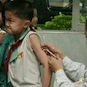
\includegraphics[width=0.18\textwidth]{kid2.jpg}
  }
  \caption{Original and cropped version of a~photo (including a~slight color variation).}
  \label{fig:cropping}  
\end{figure}

\paragraph{Camera Shots}

We have shown camera shot detection earlier in this chapter.
Different frames stemming from the same camera shot
can occur on social networks when the social networks attempt to auto-select
a~well-identifying poster frame with different heuristics,
typically resulting in different frames for different social networks.
\autoref{fig:camera-shot} shows an example of this phenomenon.

\begin{figure}[h!]
  \centering
  \subfloat[Frame 1]{
    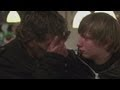
\includegraphics[width=0.2\textwidth]{camera1.jpg}
  }                
  \subfloat[Frame 2]{
    
\includegraphics[width=0.2\textwidth]{camera2.jpg}
  }
  \caption[Two different frames stemming from the same camera shot]
    {Two different frames stemming from the same camera shot,
    with the left photo appearing slightly earlier in the video.}
  \label{fig:camera-shot}  
\end{figure}

\paragraph{Aspect Ratio Changes with Bulging or Stretching}

Aspect ratio changes can either happen combined with cropping
(and thus losing parts of the photo), and/or combined with 
bulging or stretching (and thus deforming the photo).
\autoref{fig:bulged} shows an example where a~photo gets
both cropped and bulged.

\begin{figure}[h!]
  \centering
  \subfloat[Original]{
    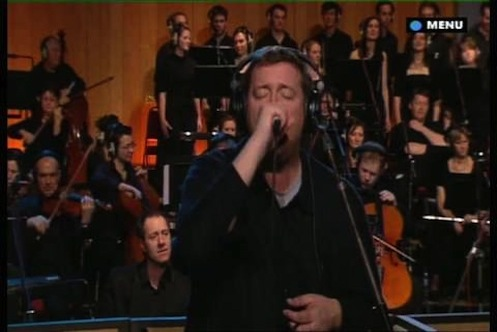
\includegraphics[width=0.225\textwidth]{singer1.jpg}
  }                
  \subfloat[Stretched and bulged]{
    
\includegraphics[width=0.3\textwidth]{singer2.jpg}
  }
  \caption{Original, and stretched and cropped version of a~photo.}
  \label{fig:bulged}  
\end{figure}

\paragraph{Photo Filters}

Especially with the popularity of Instagram, photo filters
are a~considerable reason for near-duplicate media content.
\autoref{fig:photo-filter} shows a~typical example.

\begin{figure}[h!]
  \centering
  \subfloat[Original]{
    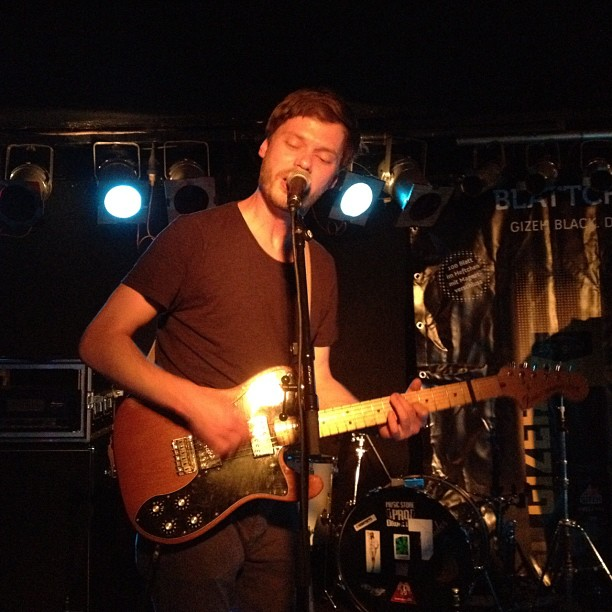
\includegraphics[width=0.2\textwidth]{clickclickdecker1.jpg}
  }                
  \subfloat[With photo filter]{
    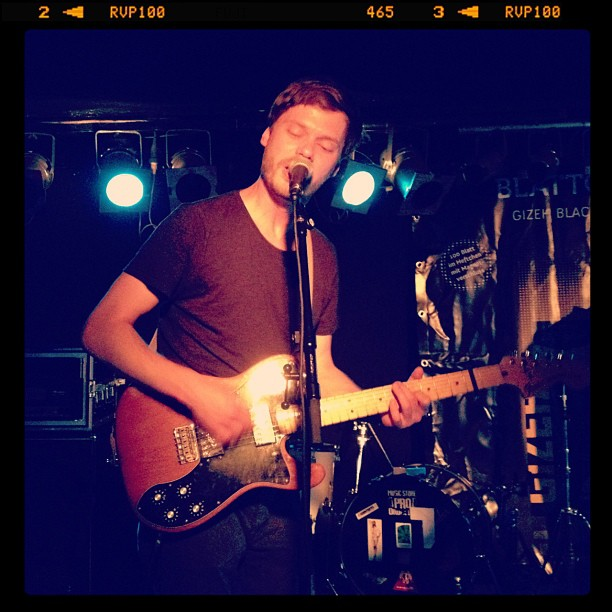
\includegraphics[width=0.2\textwidth]{clickclickdecker2.jpg}
  }
  \caption{Original, and version with an applied photo filter of a~photo.}
  \label{fig:photo-filter}  
\end{figure}

\subsection{Near-Duplicate Photo Clustering Algorithm}
\label{sec:near-duplicate-clustering-algorithm}

In this subsection, we detail our near-duplicate photo clustering algorithm
and its design goals.
We start with a~description of its face detection component.

\subsubsection{Face Detection}
\label{sec:face-detection}

Face detection is a~computer vision technology
that determines the regions of faces in photos.
Rotation-invariant face detection aims to detect faces with arbitrary
rotation angles and is crucial as the first step in automatic face detection
for general applications, as face photos are seldom upright and frontal.
Face detection is a~subclass of the broader class of object detection.
The Viola--Jones object detection framework proposed in 2001
by Paul Viola and Michael
Jones~\cite{viola2001objectdetection,viola2004robust}
provides competitive object detection rates in real-time.
It was motivated primarily by the problem of face detection.
We use a~face detection algorithm that further improves Viola--Jones,
based on work by Huang \emph{et al.}~\cite{huang2007facedetection}
and Abramson \emph{et al.}~\cite{abramson2007yef},
in a~JavaScript implementation made available by Liu~\cite{liu2012facedetection}.
This algorithm is fast enough to be applied to hundreds of photos
in well less than a~second overall processing time on a~standard laptop
(mid-2010 MacBook~Pro).

\subsubsection{Algorithm Design Goals}

In \autoref{sec:duplicate-content}, we have outlined
cases of duplicate and near-duplicate content.
Design goals of the algorithm include
the capability to detect those cases
in a~timely, entirely \emph{ad hoc} manner, without any pre-calculation.
As in general for bigger events, event coverage is exhaustive, \emph{i.e.},
there exist more media items
than one would want to watch in a~reasonable time,
it is tolerable for the algorithm to cluster media items aggressively
rather than leaving too many media items unclustered.

\subsubsection{Algorithm Description}

Our near-duplicate photo clustering algorithm belongs to the family of
tile-wise histogram-based photo clustering algorithms.
As an additional semantic feature, the algorithm detects faces
as described in \autoref{sec:face-detection}.
For two photos to be clustered,
the following conditions have to be fulfilled.

\begin{enumerate}
  \item The numbers $f_1$ and $f_2$ of detected faces in both photos
    have to be the same, ($f_1, f_2 \geq 0$).
    We note that we do \emph{not} recognize faces.
  \item Out of $m$ tiles of a~photo with $n$ tiles, ($m \leq n$),
    at most $tiles\_threshold$ tiles may differ not more than $similarity\_threshold$
    from their corresponding counterpart tiles.
\end{enumerate}

The simplified algorithm pseudocode can be seen in \autoref{code:clustering}.
In the actual implementation some speed improvements have been applied,
these were omitted in the listing for legibility reasons.
We calculate the histograms and distances only once.
The clusters are recalculated dynamically
whenever either $tiles\_threshold$ or $similarity\_threshold$ change.

\begin{lstlisting}[caption={Simplified pseudocode of the near-duplicate
    photo clustering algorithm.},
  label={code:clustering},escapechar=§]
ROWS = 10
COLS = 10
TILES_THRESHOLD = ceil(ROWS * COLS * 0.8)
SIMILARITY_THRESHOLD = 10

histograms = {}
faces = {}
for photo in photos
  faces[photo] = getFaces(photo)

  for tile in photo
    histograms[photo][tile] = getHistogram(tile)
  end for
end for  
    
distances = {}
for outerPhoto in photos
  for innerPhoto in photos
    distances[outerPhoto][innerPhoto] = {}
    for tile in histograms[outerPhoto]
      distances[outerPhoto][innerPhoto][tile] =
          abs(histograms[outerPhoto][tile] - histograms[innerPhoto][tile])
    end for
  end for
end for
  
clusters = {}
for outerPhoto in photos  
  clusters[outerPhoto] = []  
  for innerPhoto in photos
    if outerPhoto == innerPhoto continue
    
    similarTiles = 0
    distance = distances[outerPhoto][innerPhoto]
    for tile in distance      
      if distance[tile] <= SIMILARITY_THRESHOLD
        similarTiles++
      end if   
    end for
         
    if similarTiles >= TILES_THRESHOLD
      if faces[outerPhoto] == faces[innerPhoto]
        clusters[outerPhoto].push(innerPhoto)
      end if
    end if
    
  end for
end for        
\end{lstlisting}

\subsection{Experiments}

We have evaluated the near-duplicate photo clustering
on two events from recent history with high social network coverage
that we will briefly describe in the following.

\subsubsection{Grammy Awards Nominations 2013}

The Grammy Award---or short Grammy---is an award by
the National Academy of Recording Arts and Sciences of the United States
to recognize outstanding achievement in the music industry.
The annual presentation ceremony features performances by prominent artists,
and some of the awards are presented in a~widely viewed televised ceremony.
On December 5, 2012, the nominees for the 55\superscript{th} Annual Grammy Awards
were announced at an event broadcasted live by CBS
titled \emph{Grammy Nominations Concert
Live}\footnote{\url{http://en.wikipedia.org/wiki/2013_Grammy_Awards},
accessed December 7, 2012},
during which Taylor Swift and LL~Cool~J revealed the nominees in several key categories, including the so-called Big Four: Album, Record and Song of the Year and Best New Artist.
CBS suggested the hashtag \texttt{\#GRAMMYNoms} for the event.

\subsubsection{Victoria's Secret Fashion Show 2012}

The \emph{Victoria's Secret Fashion
Show}\footnote{\url{http://en.wikipedia.org/wiki/Victoria's_Secret_Fashion_Show},
accessed December 7, 2012} is an annual event
sponsored by Victoria's Secret, a~brand of lingerie and sleepwear.
The show features some of the world's leading fashion models
and is used by the brand to promote and market its goods in high-profile settings.
American network television broadcasts the show during prime time.
The show is a~lavish event with elaborate costumed lingerie and
varying music by leading entertainers
that attracts hundreds of celebrities and entertainers,
with special performers and acts every year.
The 2012 edition of the show,
which was previously taped on November 7, 2012
was aired on December 4, 2012 on CBS
to an audience of 9.48 million viewers.
CBS suggested the hashtag \texttt{\#VSFashionShow} for the event.

\subsection{Evaluation}

We have collected and made available \todo{make available}
datasets for both events with
379 photos for the \emph{Victoria's Secret Fashion Show 2012} event 
and 949 photos for the \emph{Grammy Awards Nominations 2013} event.
These photos were collected using the media item extraction framework
described in \autoref{cha:media-item-extraction}
using a~mix of hashtag searches with the official event hashtags combined
with full-text searches for event titles and variations thereof.
Due to the short-lived nature of social networks,
the returned results of the media item extraction process itself
are not reproducible, our focus in this chapter
is on media item deduplication and clustering.
The concrete clustering parameters for the algorithm were set as listed below.

\begin{small_itemize}
  \item[] $ROWS$ = $COLS$ = $5$
  \item[] $TILES\_THRESHOLD$ = $22$
  \item[] $SIMILARITY\_THRESHOLD$ = $10$
\end{small_itemize}

In the following, we discuss the clustering and deduplication results.

\section{Video Deduplication}

\subsection{Related Work}

In addition to the aforementioned  combined approach
for video and photo near-duplicate
detection~\cite{yang2009nearduplicate},
more specialized methods for video deduplication exist,
for example~\cite{min2011nearduplicatevideo,wu2009nearduplicate}
by Min \emph{et al.}\ who, given the observation that 
transformations tend to preserve the semantic information conveyed
by the video content, propose a~novel approach for identifying
near-duplicate videos by making use of both low-level visual
features and high-level semantic features
detected using trained classifiers.
Further, there is~\cite{oliveira2010nearduplicate} by Oliveira
\emph{et al.}\ who look at near-duplicate video detection
from a~human angle.  
The authors have conducted four large-scale surveys
and have confirmed that humans perceive videos as near-duplicates
both based on non-semantic features like different photo or audio
quality, but also based on semantic features like different
videos of similar content, where, according to the authors,
most research still focuses mostly on the non-semantic features.
A~survey of video deduplication methods has been conducted by
Lian \emph{et al.}\ in~\cite{lian2010survey}.

\subsection{Experiments}

\subsection{Evaluation}

\section{Conclusion}

\section*{Chapter Notes}
This chapter is partly based on the following publications:
\todo{Add publications}